\documentclass{article}
\usepackage[final]{neurips_2019}
\makeatletter
\renewcommand{\@noticestring}{11-785 Project --- Group 30, Team Support Vector. Midterm report, October 2026.}
\makeatother
\usepackage[utf8]{inputenc}
\usepackage[T1]{fontenc}
\usepackage{hyperref}
\usepackage{url}
\usepackage{booktabs}
\usepackage{amsfonts}
\usepackage{amsmath}
\usepackage{microtype}
\usepackage{graphicx}
\hypersetup{colorlinks=true,citecolor=blue,urlcolor=blue,linkcolor=blue}

\title{YOLO-CLIP: Adapting a Vision-Language Detector for Wildlife Classification at Out-of-Distribution Camera Locations}
\author{John Uzodinma \And Ramsey Njema \AND Emmilly Namuganga \And Stephen N'nouka}

\begin{document}
\maketitle

\begin{abstract}
Wildlife classifiers can struggle at camera traps absent from training---the
out-of-distribution (OOD) setting in iWildCam-WILDS. We begin by training and evaluating
implementations of published iWildCam approaches, including ResNet-50 with ABSGD and
CLIP-based FLYP and AutoFT, to establish baselines and examine different architectural
and training choices. Building on these experiments, we investigate YOLO-CLIP, an
image-level adaptation of pretrained YOLO-World. Without ground-truth bounding boxes,
we freeze the pretrained YOLO-World detector and train 181 CLIP-initialized animal-class
vectors from image-level labels using a maximum-over-regions classification loss. A
validation-selected threshold maps the top detection to an animal class or
\texttt{empty} (indicating an image without an animal). The YOLO-CLIP model achieves
20.7\% macro-F1 on familiar-camera test images and 10.7\% on unseen-camera OOD test
images. Confident wrong-species detections and frequent animal predictions on empty images reveal
limitations of this first adaptation and motivate improved region learning and
empty-class calibration we will explore further.
\end{abstract}


\section{Introduction}
Camera traps enable large-scale wildlife monitoring, but a classifier trained at one
set of locations may encounter different illumination, backgrounds, viewpoints, and
animal frequencies at new deployments \citep{beery2020iwildcam,pmlr-v139-koh21a}.
iWildCam-WILDS treats camera locations as domains and evaluates generalization to
unseen cameras as an out-of-distribution (OOD) problem. Macro-F1 is used as the main 
classification metric, which weights each class equally rather than letting frequent
classes dominate the score \citep{pmlr-v139-koh21a}.

We first implemented and evaluated established approaches: ResNet-50 with ABSGD
\citep{qi2023absgd}, CLIP-based FLYP \citep{goyal2023flyp} and AutoFT
\citep{choi2024autoft}, WiSE-FT \citep{wortsman2022wiseft}, and DFN-pretrained CLIP
\citep{fang2023dfn}. These experiments establish reference results across different
optimization, pretraining, and model-capacity choices. They also motivate a different 
question: can localized visual evidence from a vision–language detector help classify 
camera-trap images when only image-level labels are available?

We then investigate whether localized visual evidence can support image-level
recognition without bounding-box supervision. YOLO-World is an open-vocabulary
detector that associates candidate regions with text-derived class representations
\citep{cheng2024yoloworld}. Our YOLO-CLIP adaptation initializes those representations
from the 181 non-\texttt{empty} WILDS class names using CLIP \citep{radford2021learning},
freezes the pretrained detector, and trains the class vectors from image-level labels.
It produces one WILDS class prediction per image. The selected model reaches 20.7\%
ID-test and 10.7\% OOD-test macro-F1. Its errors make region learning and
empty-image calibration priorities
for the next iteration.

\section{Review of related literature}
The iWildCam-WILDS benchmark evaluates wildlife classification across camera-trap
locations, with out-of-distribution splits drawn from cameras absent from training.
Each photograph has one image-level label, including \texttt{empty} for images without
an animal. Its macro-F1 metric gives rare classes weight alongside common ones
\citep{beery2020iwildcam,pmlr-v139-koh21a}.

Our initial experiments evaluate published image-level classification approaches.
ABSGD assigns different weights to training examples to address imbalance and
difficult examples \citep{qi2023absgd}. CLIP supplies pretrained image--text
representations \citep{radford2021learning}. FLYP retains CLIP's contrastive
objective during fine-tuning, whereas AutoFT searches for a fine-tuning objective
using shifted validation data \citep{goyal2023flyp,choi2024autoft}. WiSE-FT
interpolates pretrained and fine-tuned weights, while DFN improves the data used
for CLIP pretraining \citep{wortsman2022wiseft,fang2023dfn}. These methods provide
image-level classifier baselines without explicitly selecting localized animal
evidence.

YOLIP demonstrates a related integration of detection and language-aligned wildlife
recognition. It adds a semantic proposal head to YOLOv11 and uses CLIP-based
representations to refine candidate regions in UAV imagery. Unlike our camera-trap
classification setting, YOLIP trains and evaluates a box-level detector
\citep{hu2026yolip}.

YOLO-World is the architectural basis of our YOLO-CLIP experiment. It matches
candidate regions with text-derived class representations within an integrated
detector, without requiring a separate CLIP visual-encoder pass over each detected
crop. Its original training draws on region--text pairs from annotated detection
and grounding data and from pseudo-labeled image--text data
\citep{cheng2024yoloworld}. Our adaptation instead uses iWildCam's image-level
labels to train class representations and produce one prediction per photograph,
including \texttt{empty}, without ground-truth boxes.

\section{Methodology}
\subsection{Dataset and task}
We use the official iWildCam-WILDS v2.0 classification task and its camera-location
splits \citep{beery2020iwildcam,pmlr-v139-koh21a}. The dataset contains 203,029 images
and 182 image-level classes: 181 animal labels and \texttt{empty}. The splits contain
129,809 training, 7,314 familiar-camera validation (\texttt{id\_val}), 14,961
unseen-camera validation (\texttt{val}), 8,154 familiar-camera test
(\texttt{id\_test}), and 42,791 unseen-camera test (\texttt{test}) images. We use the
dataset's own class-ID-to-name mapping. Images are converted to RGB, letterboxed to
$640\times640$ pixels, and scaled to $[0,1]$; we apply no further augmentation.
The task provides one label per image but no ground-truth animal boxes, so we do not
construct box targets.

\subsection{Model and image-level objective}
Figure~\ref{fig:architecture} shows our adaptation of the pretrained YOLO-World S-v2
detector \citep{cheng2024yoloworld}. We encode each of the 181 WILDS animal class
names with CLIP to initialize a 512-dimensional class vector
\citep{radford2021learning}. The image backbone, vision--language fusion and
localization layers remain frozen, as does the CLIP text encoder; only the class
vectors are optimized. Region-to-class matching occurs inside the detector, not
through a separate CLIP visual encoder applied to detected crops.

\begin{figure}[ht]
\centering
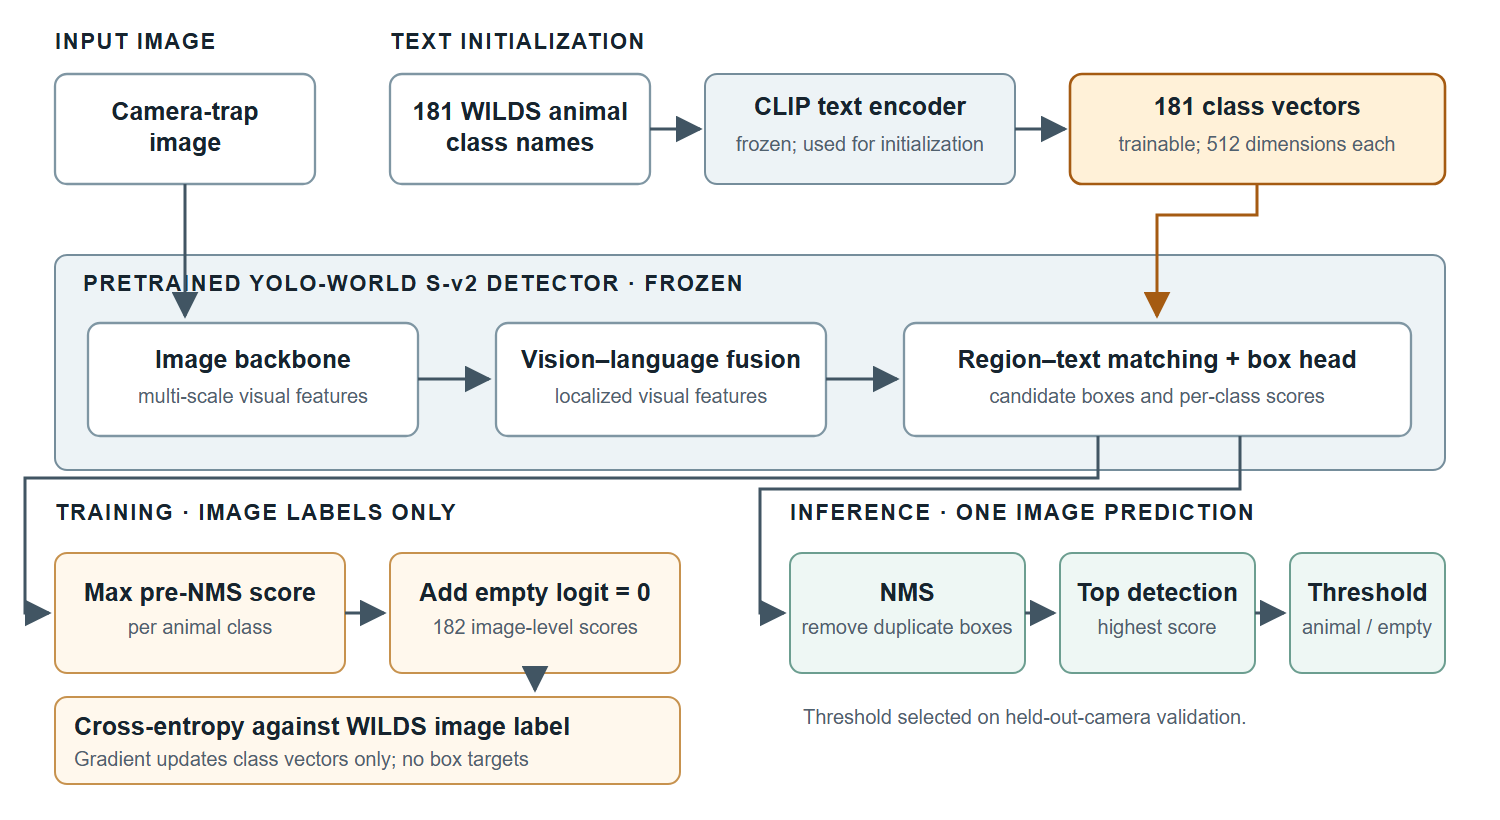
\includegraphics[width=\linewidth]{figures/yoloclip_architecture.png}
\caption{YOLO-CLIP image-level adaptation. Class-name embeddings from a frozen CLIP
text encoder initialize 181 trainable vectors; the YOLO-World detector remains frozen.
Non-maximum suppression (NMS) removes redundant overlapping detections. Training
pools the maximum region score for each animal class before NMS, appends a fixed
\texttt{empty} logit, and applies image-level cross-entropy. Inference selects the
highest-scoring detection after NMS, or \texttt{empty} below a validation-selected
threshold. No bounding-box labels or separate CLIP crop classifier are used.}
\label{fig:architecture}
\end{figure}

Let $z_{r,c}(x)$ be the raw pre-NMS score for animal class $c$ at candidate region
$r$ in image $x$. We obtain one score per animal class by taking its maximum over
regions, add a fixed \texttt{empty} logit, and minimize unweighted image-level
cross-entropy against the WILDS label $y$:
\begin{align}
s_c(x)&=\max_{r\in\mathcal R(x)} z_{r,c}(x),\quad c=1,\ldots,181,\nonumber\\
s_0(x)&=0,\qquad
\mathcal L_{\mathrm{img}}(x,y)
=-\log\frac{\exp s_y(x)}{\sum_{k=0}^{181}\exp s_k(x)}.
\end{align}
The pre-NMS scores preserve a differentiable path to the class vectors; neither
hard confidence filtering nor NMS is part of the training loss. This objective
does not assert that an image contains only one animal or identify its true box.

\subsection{Training and model selection}
We train for 20 epochs with AdamW, batch size 16, constant learning rate $10^{-4}$,
zero weight decay, gradient-norm clipping at 1, and seed 785. A two-image
animal/\texttt{empty} smoke test confirmed that the loss updates only the class
vectors and that a tiny subset can be fitted before the full run. The initial
five-epoch run was extended to 20 epochs by resuming the class vectors and optimizer
state rather than restarting training. After each epoch, we compute image-level
cross-entropy on \texttt{id\_val} and select the checkpoint with the lowest value.

\subsection{Inference and evaluation}
At inference, NMS removes overlapping detections. We use
an NMS confidence floor of 0.001, intersection-over-union threshold of 0.7, and cap
of 20 boxes per image. The class of the highest-scoring remaining detection becomes
the image prediction; if there is no detection or its score is below a threshold,
we predict \texttt{empty}. We choose that threshold on \texttt{val} by maximizing
the official WILDS macro-F1 and then freeze it with the selected checkpoint before
evaluating \texttt{id\_test} and \texttt{test}. Thus, the threshold-tuned
\texttt{val} score is a selection result, not an independent test estimate.

Our primary metric is the official image-level macro-F1, which gives equal weight
to classes rather than allowing common classes to dominate. We report average
accuracy, macro recall, and the fraction predicted \texttt{empty} as diagnostics.
The pre-NMS training scores and post-NMS inference confidences are not identical;
we retain this distinction when interpreting errors. We do not report detection
mean average precision because WILDS does not supply box annotations.

\section{Baseline Experiments}
\subsection{Classifier baselines}
We implemented several published iWildCam approaches to establish how different
model and training choices perform under the same camera-location shift. Zero-shot
CLIP ViT-B/16 measures transfer without wildlife fine-tuning
\citep{radford2021learning}. ResNet-50 with ABSGD provides a supervised
convolutional reference, while FLYP and AutoFT examine different ways to adapt CLIP
ViT-B/16 \citep{he2015resnet,qi2023absgd,goyal2023flyp,choi2024autoft}. Our AutoFT run
uses published settings rather than reproducing the paper's full objective search.
We also evaluate WiSE-FT weight interpolation and a larger DFN-pretrained CLIP
ViT-H/14 model \citep{wortsman2022wiseft,fang2023dfn}. These are our measured
implementations, not numbers copied from the leaderboard. Because backbone,
pretraining, resolution, seed, and training recipe differ across runs, their scores
provide context rather than an isolated test of any one design choice.

\subsection{Frozen detector reference}
The closest architectural reference for YOLO-CLIP is our frozen, prompted YOLO-World
run. It uses the same pretrained detector and WILDS animal names, then converts the
highest-scoring detection into one image label, predicting \texttt{empty} below a
validation-selected threshold. We evaluated this reference on validation data
before training class vectors. It checks the label mapping and image-level
prediction rule, but is not the central experiment or an independent test
benchmark. The trained YOLO-CLIP run retains the detector and prediction rule
while adapting class vectors from WILDS image labels; it selects its own threshold
on validation data.

\section{Initial Results and Findings}
\begin{table}[ht]
\centering
\small
\begin{tabular}{lrrrr}
\toprule
Model & IDVal & IDTest & OODVal & OODTest \\
\midrule
Zero-shot CLIP ViT-B/16 & 8.8 & 8.7 & 12.3 & 11.0 \\
ResNet-50 + ABSGD (fixed-norm) & -- & 49.4 & -- & 33.9 \\
FLYP ViT-B/16 & 43.2 & 49.3 & 32.9 & 30.8 \\
AutoFT ViT-B/16 & 49.4 & 43.4 & 39.1 & 34.8 \\
AutoFT + WiSE-FT ViT-B/16 & 49.8 & 47.1 & 40.2 & 37.1 \\
DFN CLIP ViT-H/14 & 56.4 & 59.7 & 50.3 & 45.7 \\
\midrule
Frozen YOLO-World reference & 2.45 & -- & 2.24\textsuperscript{*} & -- \\
\textbf{YOLO-CLIP} & -- & 20.7 & 16.0\textsuperscript{*} & 10.7 \\
\bottomrule
\end{tabular}

\caption{Image-level macro-F1 (\%). ID and OOD denote familiar and unseen camera
locations. The fixed-norm ResNet result is a three-seed mean; the other trained
classifier results are single runs. The YOLO-CLIP checkpoint was selected on IDVal
cross-entropy. Asterisks mark OODVal scores used to select each detector's
\texttt{empty} threshold, so they are tuning scores rather than independent
evaluations. Dashes denote unmeasured splits.}
\label{tab:baselines}
\end{table}

\paragraph{Classifier baselines.}
Table~\ref{tab:baselines} reports our implementations of published classifier
approaches alongside the detector-based experiments. Among the trained classifiers,
DFN CLIP ViT-H/14 has the highest OOD-test macro-F1 at 45.7\%, followed by AutoFT
with WiSE-FT at 37.1\%. The fixed-norm ResNet-50 reaches 33.9\%, while zero-shot
CLIP ViT-B/16 reaches 11.0\%. DFN declines from 59.7\% on IDTest to 45.7\% on
OODTest. Because backbone, pretraining, resolution, and training recipes differ,
these comparisons describe the observed runs rather than isolate any single design
choice. The main YOLO-CLIP training history is shown in
Figure~\ref{fig:training}.

\begin{figure}[ht]
\centering
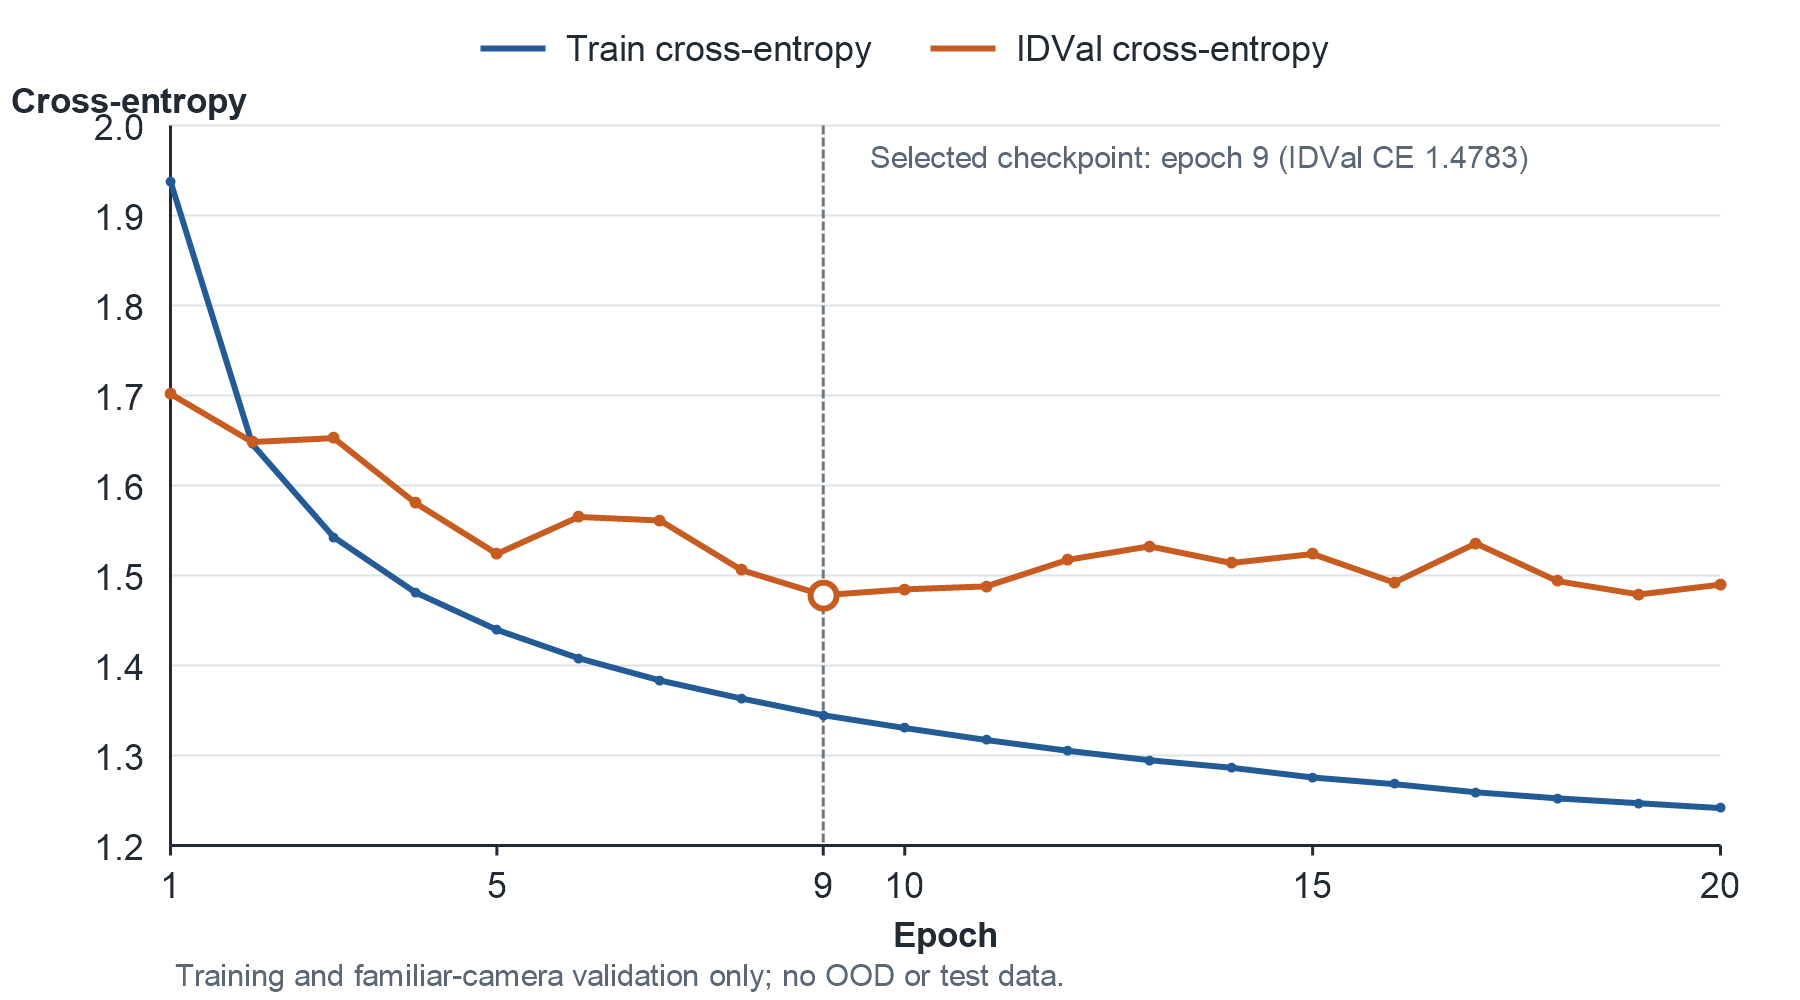
\includegraphics[width=\linewidth]{figures/yoloclip_training_curves.png}
\caption{YOLO-CLIP image-level cross-entropy over 20 epochs. Training loss declines
throughout, while familiar-camera validation (\texttt{id\_val}) loss is lowest at
epoch 9 (1.4783), the checkpoint selected before threshold tuning. No
held-out-camera validation or test data enter these curves.}
\label{fig:training}
\end{figure}

\paragraph{YOLO-CLIP training and validation.}
The image-level training cross-entropy fell from 1.9377 after epoch 1 to 1.2417
after epoch 20. IDVal cross-entropy was lowest at epoch 9 (1.4783), which we
selected before tuning the \texttt{empty} threshold; it was 1.4901 at epoch 20.
On held-out-camera validation, the selected model obtained 16.0\% macro-F1 with
its validation-tuned threshold, compared with 2.24\% for the frozen YOLO-World
reference with its own tuned threshold. These are selection-set scores, not
independent test results.

\paragraph{Final test results.}
We fixed the epoch-9 checkpoint, post-NMS image rule, and validation-selected
threshold (0.080436) before evaluating either final test split. YOLO-CLIP reached
20.7\% macro-F1 on IDTest and 10.7\% on OODTest. Its corresponding accuracies were
47.3\% and 49.2\%, illustrating why accuracy alone is insufficient for the
imbalanced 182-class task.

\paragraph{Observed failure patterns.}
On OODVal, 16.0\% of images were labeled \texttt{empty}, but the trained model
predicted \texttt{empty} for 11.0\%; on OODTest those fractions were 33.0\% and
20.2\%. This mismatch suggests imperfect empty-class calibration, although it
does not by itself identify the cause of individual errors. Inspection also showed
confident wrong-species detections. Since the visual detector was frozen and
training used no box targets, adapting class vectors alone could not correct a
region the detector failed to localize.

\section{Discussion}
On OODVal, the trained model obtains higher macro-F1 than the frozen YOLO-World
reference, suggesting that image labels can help adapt class matching without
box supervision. OOD-test macro-F1 is 10.7\%. The IDTest--OODTest gap of
10.0 percentage points is consistent with camera-location shift remaining
difficult, although these aggregate results do not isolate its effect from
differences in species frequencies and image conditions.

Several design choices may limit this adaptation. Only the class vectors learn;
the visual backbone, region proposals, and localization remain fixed. Maximum
pre-NMS pooling lets one region dominate each class's training score, but does not
establish whether that region contains the labeled animal. Inference instead uses
the top post-NMS detection. The fixed \texttt{empty} training logit and separately
tuned inference threshold create a further mismatch. The observed shortfall in
predicted \texttt{empty} images is consistent with calibration error, but a new
threshold cannot repair missed animals or confident wrong-species detections.
Class imbalance also makes accuracy a poor substitute for macro-F1.

\section{Planned Work}
We plan to explore both smaller extensions to the current YOLO-World baseline and a
more involved YOLO--CLIP fusion architecture. Validation error analysis will
distinguish wrong-species matches, missed or false regions, and
\texttt{empty}-decision errors before we select variants.
\begin{enumerate}
\item Test a trainable \texttt{empty} bias or small image-level calibrator against
the present threshold-only rule. We will specify how training-time pre-NMS scores
relate to the post-NMS inference decision and compare macro-F1 and
empty/non-empty errors on validation data.
\item Test smoother or attention-based region aggregation in place of hard
max-pooling, and limited fine-tuning of the semantic matching head or
vision--language fusion layers. We will ablate these changes separately, initially
retaining the pretrained backbone and localization branch, to assess whether
better use of candidate regions improves species matching.
\item Investigate a more involved architecture built around a base YOLO detector
and a trainable interface to CLIP representations. Candidate designs include
projecting localized YOLO features toward CLIP class-name embeddings and, possibly,
proposal-level CLIP visual processing inspired by YOLIP \citep{hu2026yolip}.
The exact fusion and training objective remain open: WILDS supplies image labels,
not box targets, and the system must still produce one image-level class.
\end{enumerate}
We will compare each variant with the unchanged baseline using training and
validation data. Because the final-test results have already been viewed, they
will not be used to tune these extensions or described as fresh, untouched tests.

\paragraph{Team contributions.}
Ramsey Njema developed the AutoFT/WiSE-FT lane; Stephen N'nouka ran FLYP; Emmilly
Namuganga ran ResNet/DFN. John Uzodinma developed and evaluated the YOLO-CLIP
adaptation. Further extensions and the comparative analysis will be shared across
the team.

\noindent\textbf{GitHub:}
\url{https://github.com/rnjema/idl-f26-g30-project}

\bibliographystyle{plainnat}
\bibliography{references}
\end{document}
